\documentclass[a4paper]{article}

\usepackage[T1]{fontenc}
\usepackage{textcomp}
\usepackage{mathtools,amssymb,amsthm}
\usepackage[hmargin=1in,vmargin=1in]{geometry}
\usepackage{graphicx,cancel}
\usepackage[math-style=TeX]{unicode-math}
% \usepackage[lite,subscriptcorrection,nofontinfo]{mtpro2}
\usepackage{fontspec}
\usepackage[colorlinks=true,allcolors=blue]{hyperref}

\defaultfontfeatures{Ligatures=TeX,Numbers=OldStyle}
\setmainfont{Palatino Linotype}
\setmathfont{TeX Gyre Pagella Math}
%\usepackage[integrals]{wasysym}
\frenchspacing

\newcommand*{\parasp}{\setlength{\parskip}{10pt plus 2pt minus 3pt}}
\newcommand*{\noparasp}{\setlength{\parskip}{0pt plus 1pt}}
\newcommand*{\setparasp}[1]{\setlength{\parskip}{#1}}
\newcommand*{\pskip}{\vskip 10pt plus 2pt minus 3pt}
\newcommand\LEFTRIGHT[3]{\left#1 #3 \right#2}
\newcommand*{\paren}[1]{\LEFTRIGHT(){#1}}
\newcommand*{\brkt}[1]{\LEFTRIGHT[]{#1}}
\newcommand*{\unit}[1]{\,\mathrm{#1}}
\newcommand*{\DeclareUnit}[2]{\newcommand*{#1}{\unit{#2}}}
\DeclareUnit{\cm}{cm}
% \renewcommand*{\m}{\unit{m}}
\DeclareUnit{\m}{m}
\DeclareUnit{\kg}{kg}
\DeclareUnit{\s}{s}
\newcommand*{\R}{\mathbb{R}}
\newcommand*{\Rp}{(0,+\infty)}
\newcommand*{\Rm}{(-\infty,0)}
\newcommand*{\deduce}{\mathrel{\Downarrow}}
\newcommand*{\abs}[1]{\left\lvert #1 \right\rvert}
\newcommand*{\reason}[1]{\langle \, \text{#1} \, \rangle}

\newcounter{ListCounter}
\newenvironment{enumerate*}%
{\begin{list}%
        {\arabic{ListCounter}.}%
        {\usecounter{ListCounter}%
            \setlength{\topsep}{1.5pt}%
            \setlength{\itemsep}{1.5pt} } }%
    {\end{list}}

\DeclareMathOperator{\arccosh}{arccosh}
\DeclareMathOperator{\gammaf}{\Gamma}
\DeclareMathOperator{\var}{var}
\DeclareMathOperator{\Ber}{Bernoulli}
\DeclareMathOperator{\Cov}{Cov}
\DeclareMathOperator{\E}{E}
%\newcommand*{\diff}{\mathop{}\!d}
\newcommand*{\diff}{\mathop{}\!\mathit{d}}
%\newcommand*{\diff}{\mathop{}\!\mathrm{d}}
\newcommand*{\dx}{\diff x}
\newcommand*{\dy}{\diff y}
\newcommand*{\dz}{\diff z}
\newcommand*{\dt}{\diff t}
\newcommand*{\du}{\diff u}
\newcommand*{\dv}{\diff v}
\newcommand*{\dtheta}{\diff \theta}
\newcommand*{\ddx}{\frac{\diff}{\dx}}
\newcommand*{\fwdf}{\mathop{}\!\Delta}
\newcommand*{\dydx}{\frac\dy\dx}
\newcommand*{\pdpdx}{\frac\partial{\partial x}}
\newcommand*{\pdpdy}{\frac\partial{\partial y}}
\newcommand*{\pdpdz}{\frac\partial{\partial z}}
\newcommand*{\pdpdu}{\frac\partial{\partial u}}
\newcommand*{\pdpdv}{\frac\partial{\partial v}}
\newcommand*{\pdpdt}{\frac\partial{\partial t}}
\newcommand*{\pdzpdx}{\frac{\partial z}{\partial x}}
\newcommand*{\pdzpdy}{\frac{\partial z}{\partial y}}
\newcommand*{\pdzpdt}{\frac{\partial z}{\partial t}}
\newcommand*{\pdxpdt}{\frac{\partial x}{\partial t}}
\newcommand*{\pdypdt}{\frac{\partial y}{\partial t}}

\AtBeginDocument{%
	\renewcommand{\perp}{\mathrel{\bot}}
	\let\leq\leqslant
	\let\le\leq
        \let\geq\geqslant
        \let\ge\geq}

\newcommand*{\Prb}[1]{\section*{Problem #1}}
\newcommand{\Q}[1]{\textbf{Question:} #1}
\newcommand*{\A}[1]{\textbf{Answer:} #1}
\newcommand{\Prblm}[3]{\Prb{#1} \Q{#2} \\[6pt] \A{#3}}


\begin{document}
    \Prblm{1}{$ \frac{d}{dx} \int_{t=0}^{\arcsin x} \ln \left| \sin t + \cos t
                \right| \, dt $.}
    {$ \frac{1}{\sqrt{1-x^2}}\ln \left| x + \sqrt{1-x^2} \right| $.}
    
    \begin{align*}
    \frac{d}{dx} \int_{t=0}^{\arcsin x} \ln \left| \sin t + \cos t \right| \, dt
        &= \frac{d}{dx} \int_{t=0}^{u} \ln \left| \sin t + \cos t
            \right| \, dt
            && \reason{$ u = \arcsin x $} \\
        &= \ln |\sin u + \cos u| \cdot \frac{du}{dx}
            && \reason{$\textstyle \frac{d}{dx} \int_{t=a}^{u(x)} f(t) \,dt =
                        f(u(x)) \frac{du(x)}{dx} $} \\
        &= \frac{\ln |x + \cos(\arcsin x)|}{\sqrt{1-x^2}}
            && \reason{$ u = \arcsin x $ and evaluate $ \tfrac{du}{dx} $} \\
        &= \frac{\ln |x + \sqrt{1-x^2}|}{\sqrt{1-x^2}}
            && \reason{$ \cos(\arcsin x) = \sqrt{1-x^2} $}
    \end{align*}
    
    \Prblm{2}{$ \frac{d}{dx} \int_{t=\sin x}^{\tan x} e^{-t^2} \, dt $.}
    {$ e^{-\tan^2 x} \cdot \sec^2 x - e^{-\sin^2 x} \cdot \cos x $.}
    
    \begin{align*}
    \frac{d}{dx} \int_{t=\sin x}^{\tan x} e^{-t^2} \, dt
        &= \frac{d}{dx} \paren{\int_{t=0}^{\tan x} e^{-t^2} \, dt -
            \int_{t=0}^{\sin x} e^{-t^2} \, dt}
            && \reason{additivity} \\
        &= \frac{d}{dx} \int_{t=0}^{\tan x} e^{-t^2} \, dt
            - \frac{d}{dx} \int_{t=0}^{\sin x} e^{-t^2} \, dt
            && \reason{linearity} \\
        &= e^{-\tan^2 x} \cdot \sec^2 x - e^{-\sin^2 x} \cdot \cos x.
            && \reason{$\textstyle \frac{d}{dx} \int_{t=a}^{u(x)} f(t) \,dt =
                f(u(x)) \frac{du(x)}{dx} $} \\
    \end{align*}
    
    \Prblm{3}
    {Which of the following is the leading order term in the Taylor series about
    $ x=0 $ of
        \[ f(x) = \int_{t=0}^x\ln(\cosh t) \, dt \]
    \textbf{Hint:} yes, there's more than one way to do this problem\dots\ Try
    using the F.T.I.C. to compute the derivatives.}
    {$ \frac{x^3}{3!} = \frac{x^3}6 $.}
    
    \parasp
    The constant term of the Taylor series must be zero since $\textstyle f(0) =
    \int_{t=0}^0 x\ln(\cosh t) \, dt $. So if the first derivative at $ x=0 $ is
    nonzero, then $ f'(0)\cdot x $ must be the leading order term. And
        \[ \frac{d}{dx} f(x) = \frac{d}{dx} \int_{t=0}^x\ln(\cosh t) \, dt
                             = \ln(\cosh x)\,, \]
    so $ f'(0) = \ln(\cosh 0) = \ln 1 = 0 $. Oops, we have to take the second
    derivative at $ x=0 $,
        \[ \frac{d^2}{dx^2} f(x) = \frac{d}{dx} \ln(\cosh x)
                                 = \frac{\sinh x}{\cosh x}\,, \]
    so $ f''(0) = \sinh 0 / \cosh 0 = 0 $. Oops again, let's take the third derivative,
        \[ \frac{d^3}{dx^3} f(x) = \frac{d}{dx} \frac{\sinh x}{\cosh x}
                                 = \frac{1}{\cosh^2 x}\,, \]
    so $ f'''(0) = 1 $. Thus, the leading order term is
        \[ \frac{x^3}{3!} = \frac{x^3}6. \]
    
    \Prblm{4}
    {We usually use Riemann sums to approximate integrals, but we can go the
    other way, too, using an antiderivative to approximate a sum. Using only
    your head (no paper, no calculator), tell me which of the following is the
    best estimate for
        \[ \sum_{n=0}^{100} n^3. \]}
    {$ 2.5\times 10^7 $.}
    
    \begin{align*}
        \sum_{n=0}^{100} n^3
            &\approx \int_0^{100} x^3 \, dx \\
            &= 100^4/4 \\
            &= 2.5\times 10^7
    \end{align*}
    
    \begin{figure}[h]
    \centering
    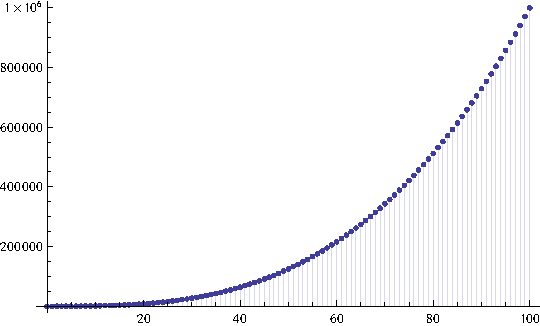
\includegraphics[width=0.7\linewidth]{hw26_challenge_fig1}
    \label{fig:hw26_challenge_fig1}
    \end{figure}

\end{document}